%!TEX root = ../../main.tex
\section{Hardware} % (fold)
\label{sec:mr_hardware}

\textbf{Provided hardware}
\\
\\
The platform for the mobile robot revolves around the SDU FrobitPro wheeled 
robot, mounted with a tip loading platform. The whole system is driven 
by a micro-atx computer system with Ubuntu 14.04 and Ros indigo to form the 
Frobomind system. As power source is a 12V 7000mAh lead battery (same type as 
used for 
small mopeds) and a SDU Frobomind controller, that also act as a controller for 
the driving motors. To enable a continous operation of the mobile robot, an 
intelligent CTEK 5.0A charger was used. This provided enough charging 
capability to test the system for an indefinite time while connected.\\ An 
overview of the robot can be seen in Figure \ref{fig:frobit}.It was arbitrarily 
chosen that the front of the robot would be in the end with the small wheel.\\
\begin{figure}[H]
	\centering
	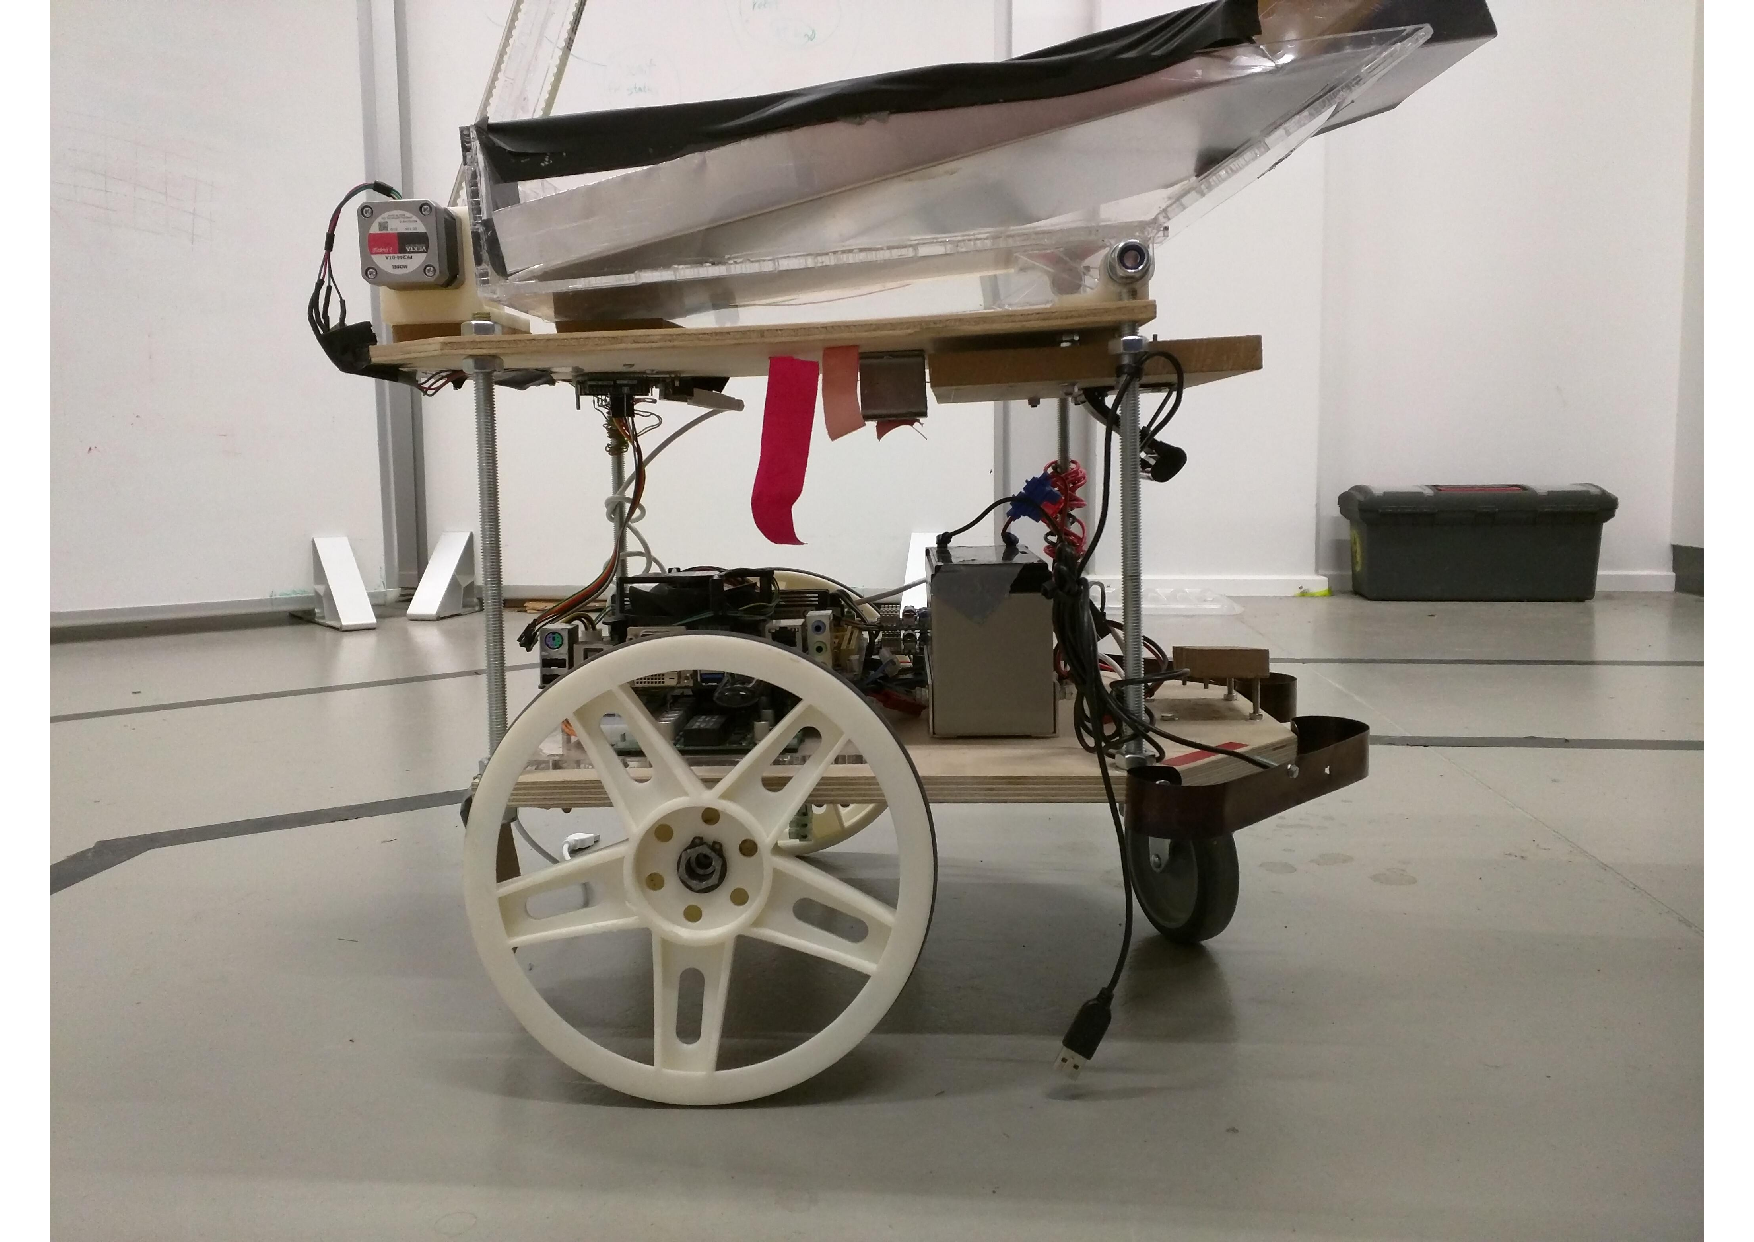
\includegraphics[width=0.7\textwidth]{frobit_profile}
	\caption{FrobitPro Robot}
	\label{fig:frobit}
	\end{figure}
\textbf{The main components for the tipper:}
\begin{itemize}
	\item PK-244-01A Bipolar Stepper motor
	\item Arduino UNO
	\item L298N dual H-bridge control board (Self-obtained)
	\item 2x Microswitch w/arm as end-point sensors for the motion
\end{itemize}   

To obtain valuable information about the surrounding environment, following 
sensors were used:\\
\begin{itemize}
	\item Sick LIDAR laser scanner
	\item VectorNav	 IMU
	\item Logitech Webcam
\end{itemize} 

The use of these sensors will be described in the appropriate sections. The IMU 
and LIDAR was on lend from the student library.\\
\\
\textbf{Modifications}\\
Along the development and testing phase of the project it was discovered that 
custom hardware modifications was necessary for the sensors to be mounted 
properly to the robot, in regards to protection of the sensors and be able to 
make proper use of these. A quick sum-up of these modifications can be seen in 
the following figures:\\

It was decided pre-hand that it was not allowed to make adjustments(e.g. 
cutting and drilling) in the base plate of the robot, of which it was chosen 
that the line-following camera would be mounted below the tipper without 
obstructing the LIDAR's field of view. This can be seen on \ref{fig:webcam_mr}.
\begin{figure}[H]
	\centering
	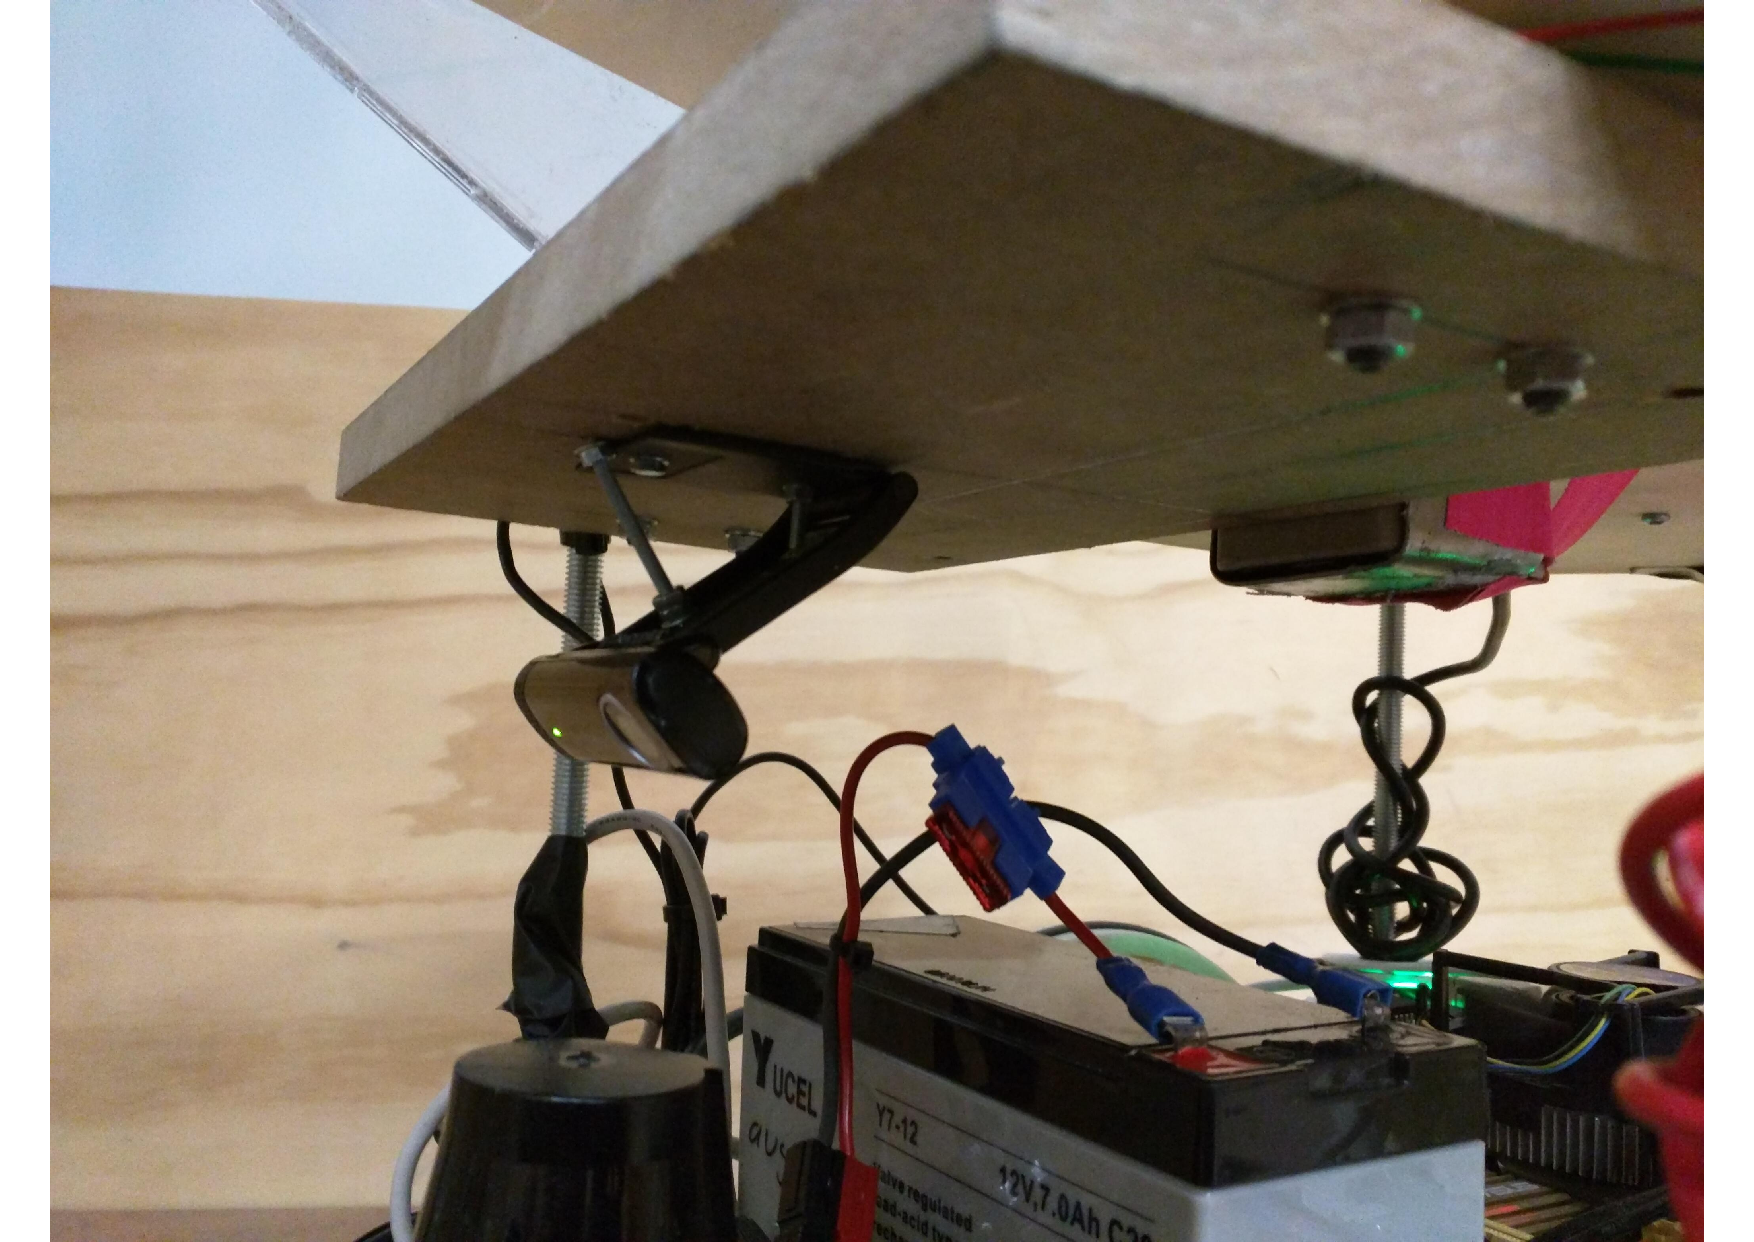
\includegraphics[width=0.7\textwidth]{webcam_mr}
	\caption{Line-following/QR detection camera}
	\label{fig:webcam_mr}
	\end{figure}
The previous use of an IMU on the robot had a remaining mount. With duct tape 
this was firmly attached. This can also be seen in figure \ref{fig:webcam_mr} 
in the background.
\begin{figure}[H]
	\centering
	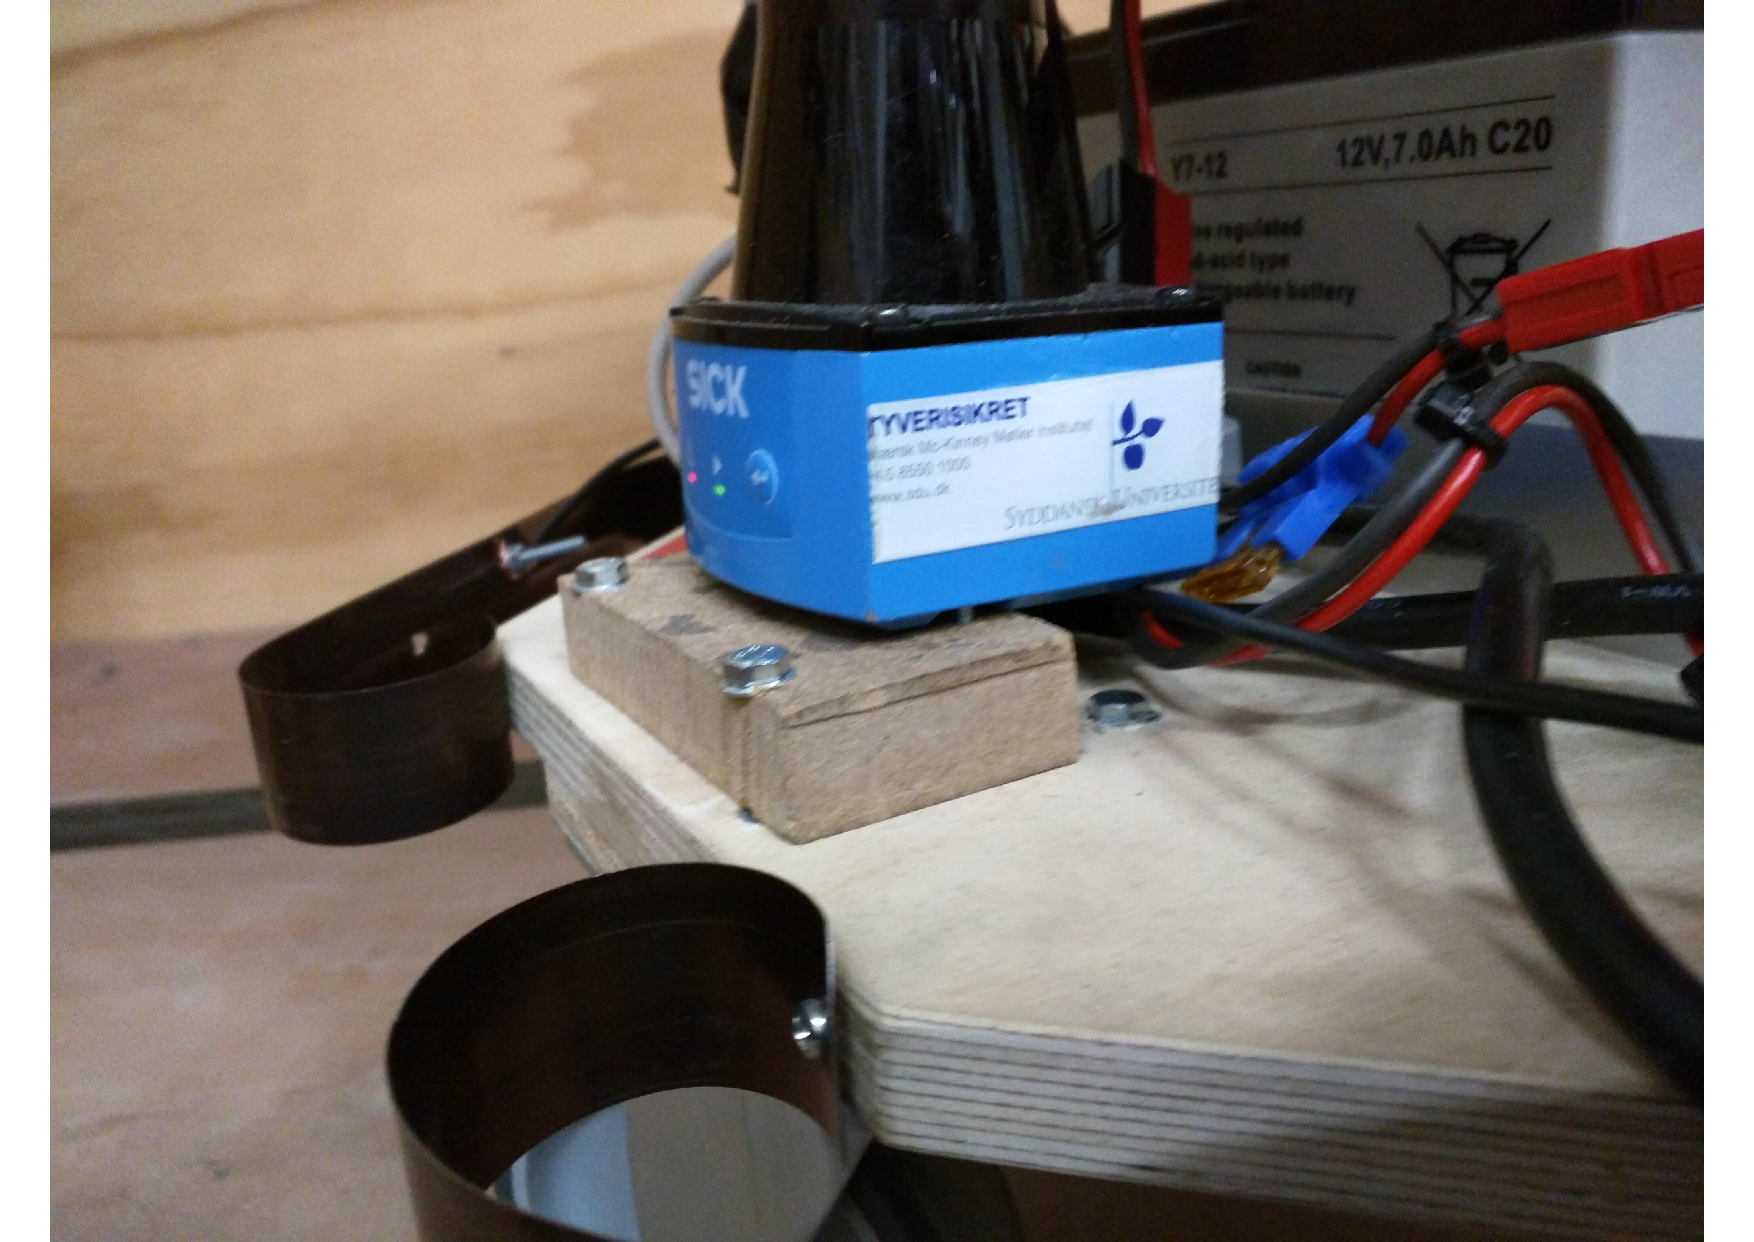
\includegraphics[width=0.7\textwidth]{lidar}
	\caption{Lidar laser scanner}
	\label{fig:lidar}
\end{figure}

In the preliminary tests, the Lidar was put on a wooden board in front of the 
robot. This to get as much use of the 270 degrees sensor angles as possible. 
Experimentally and in regards to the price of this sensor, it was later chosen 
to move it within the robot base to avoid any mishaps during an unforseen 
collision. This obviously sacrified the viewing angle.
\ref{fig:lidar}

The arduino and H-bridge for the tipper control was mounted close to the 
stepper motor as shown in \ref{fig:arduino}. After some 
testing/collisions with the other robots, the usb plug of the arduino board had 
to be reattached and the board was therefore moved so nothing would interfere 
with the usb plug during runs. 

\begin{figure}[H]
	\centering
	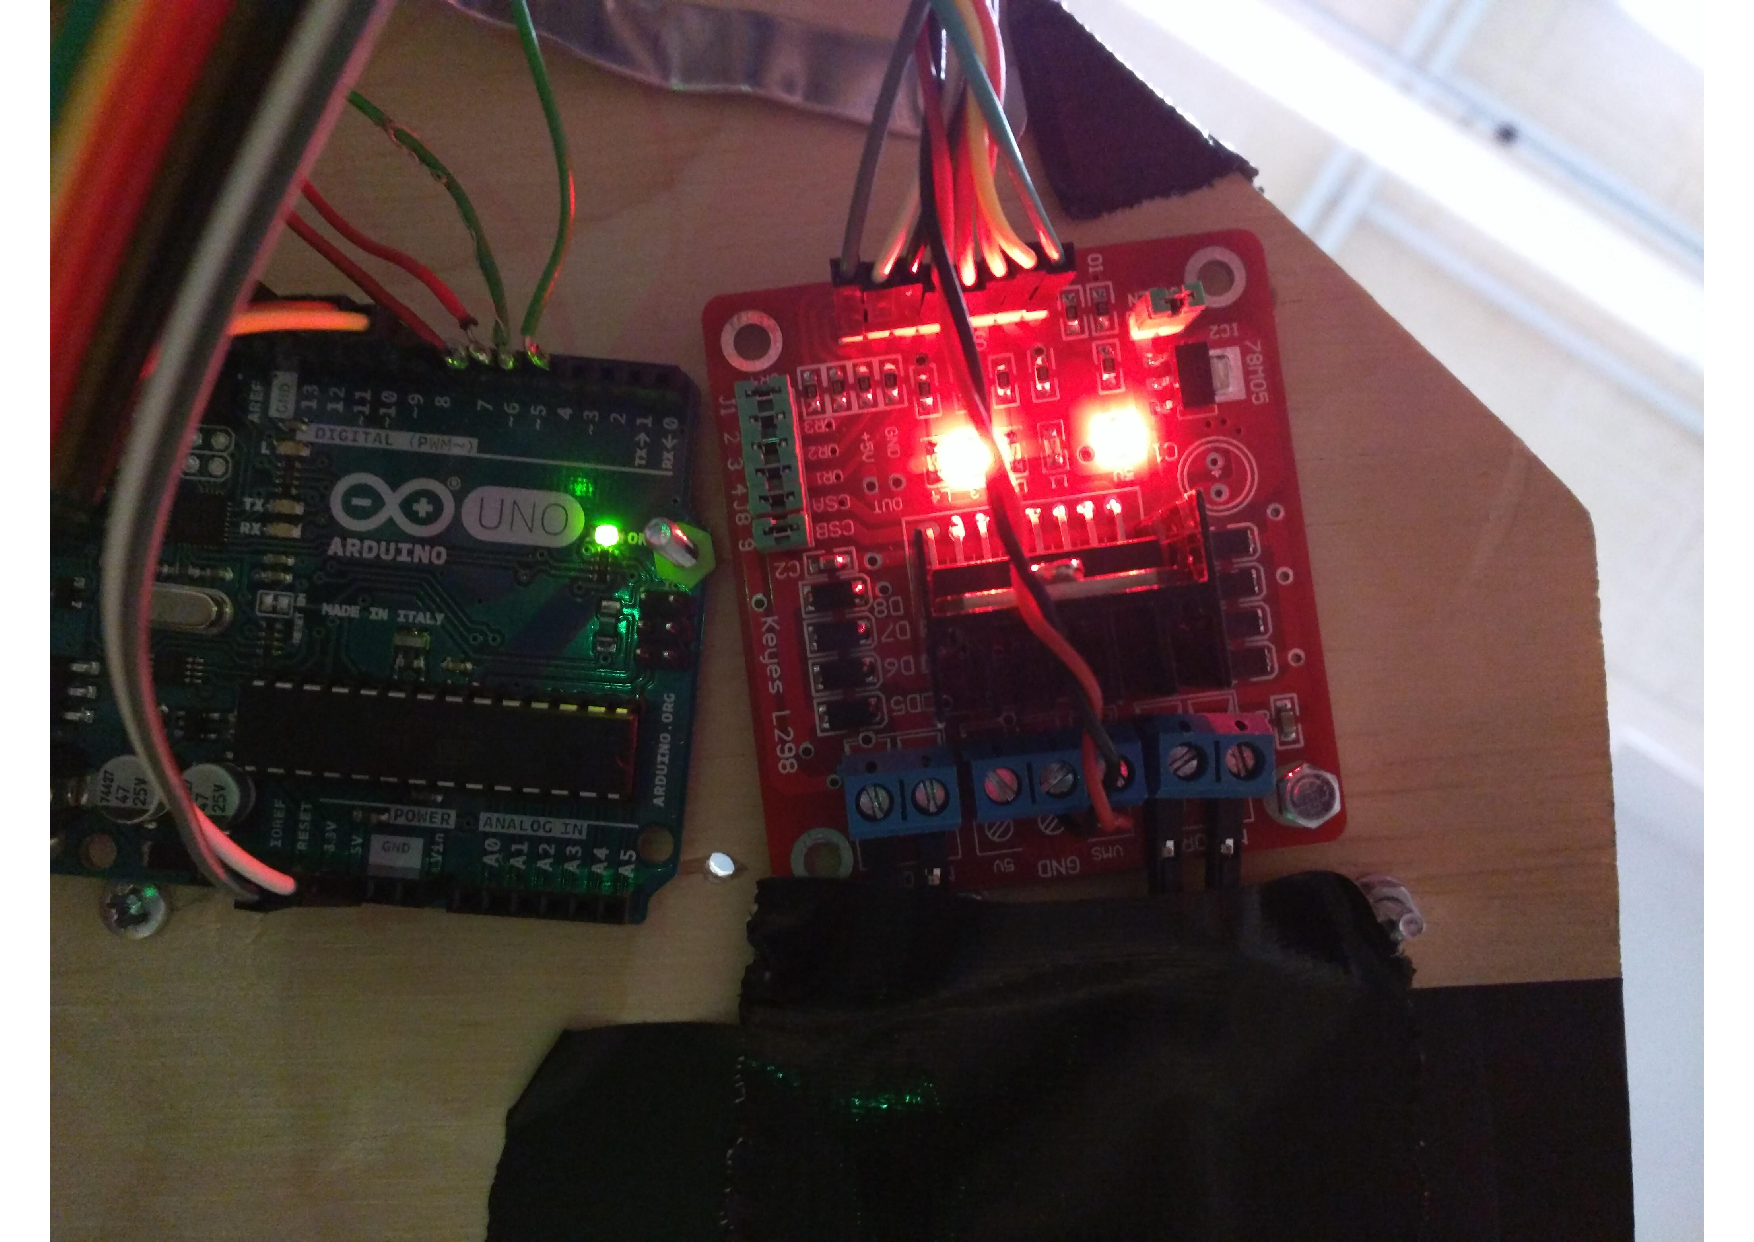
\includegraphics[width=0.7\textwidth]{arduinoandhbridge}
	\caption{Arduino and H-bridge mounted on the robot}
	\label{fig:arduino}
\end{figure}

During docking sessions in the dispenser/charging station, it was discovered 
that attaching a bumper-like system would increase the angle of which the robot 
could enter the charging station thus reducing the strictness of localization 
for going to the charger. The bumper idea can be seen in 
\ref{fig:bumper}.  


\begin{figure}[H]
	\centering
	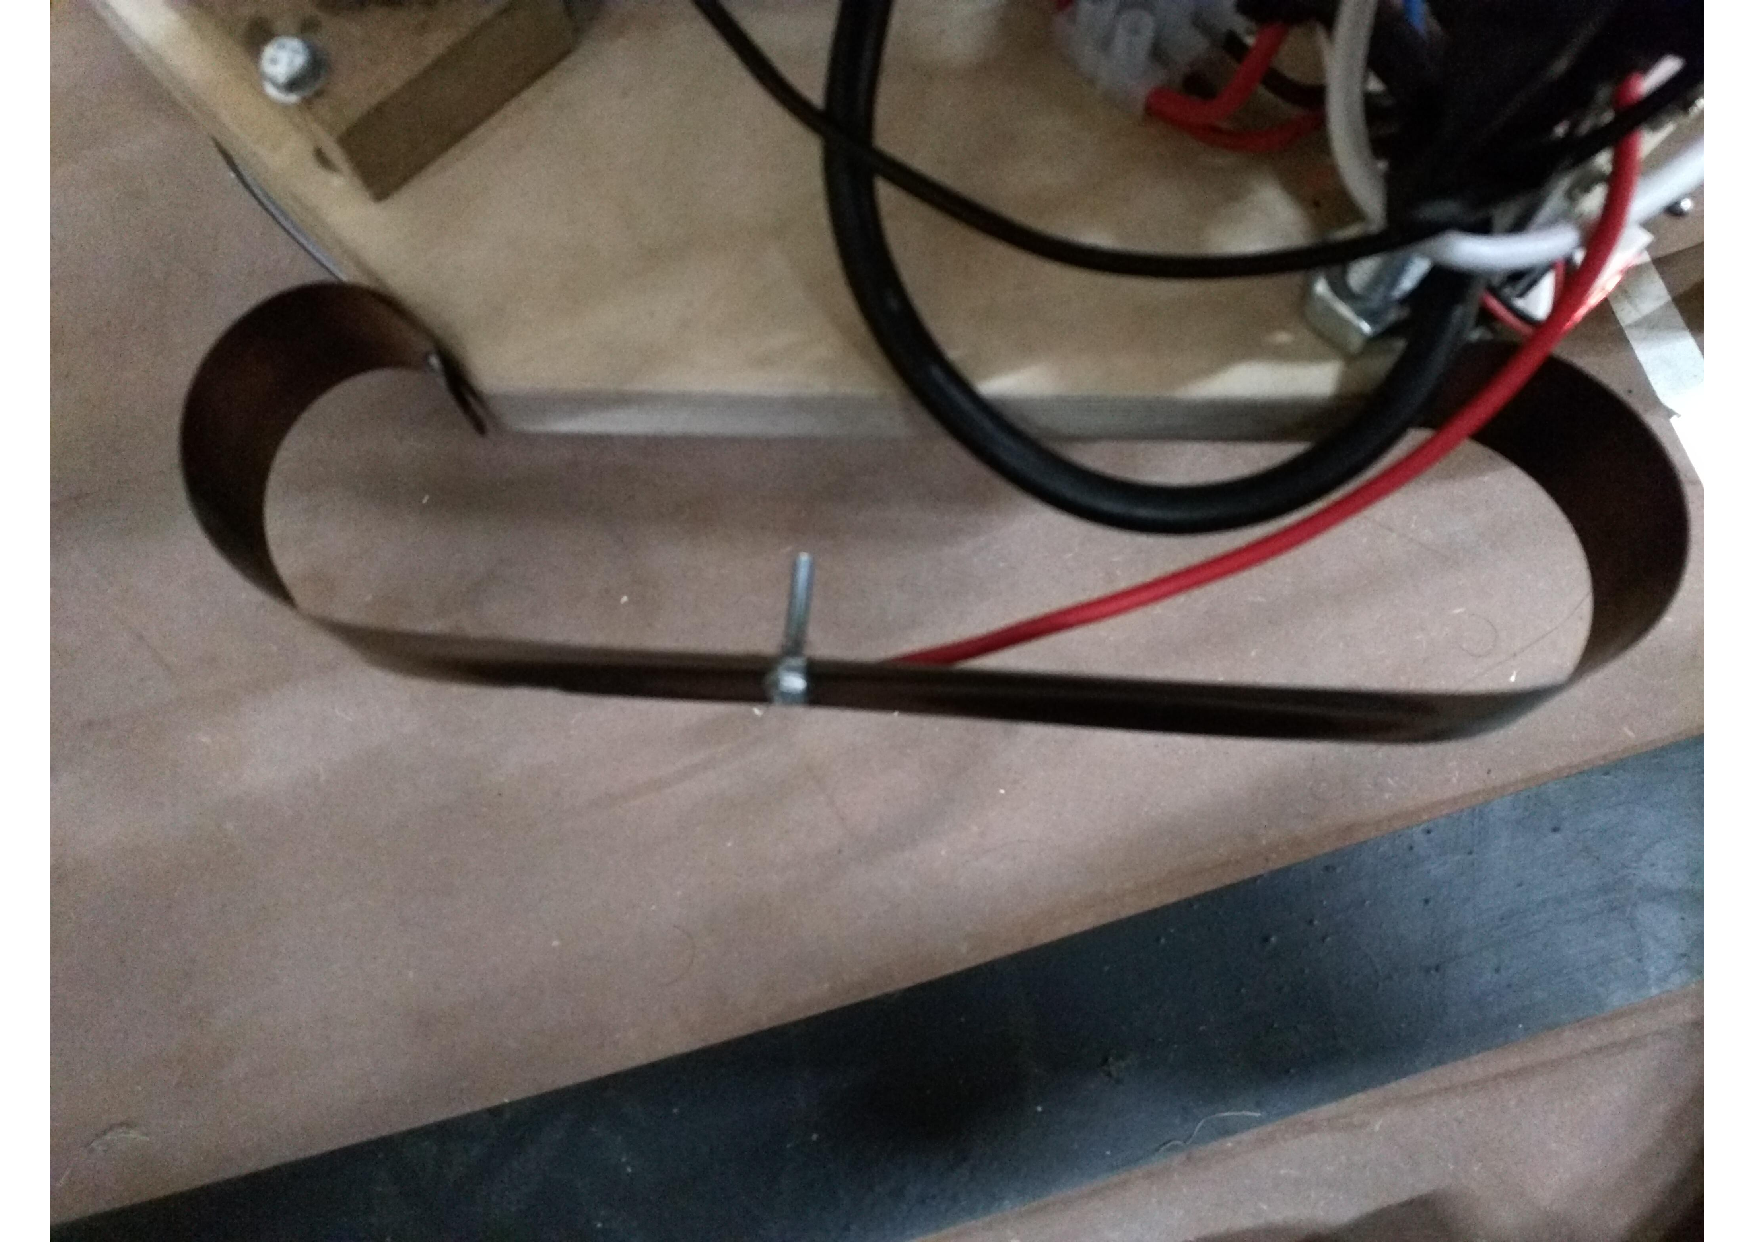
\includegraphics[width=0.7\textwidth]{bumper_mr}
	\caption{Bumper on the Mobile robot}
	\label{fig:bumper}
\end{figure}
Finally the plexiglas tray on top of the robot was found inadequate to deliver 
all bricks at the conveyor belt, so an aluminium insert was created. To ensure 
that the bricks were delivered to the conveyor belt and not next to it, this 
insert was created with a narrow tip, as seen in \ref{fig:tray}

\begin{figure}[H]
	\centering
	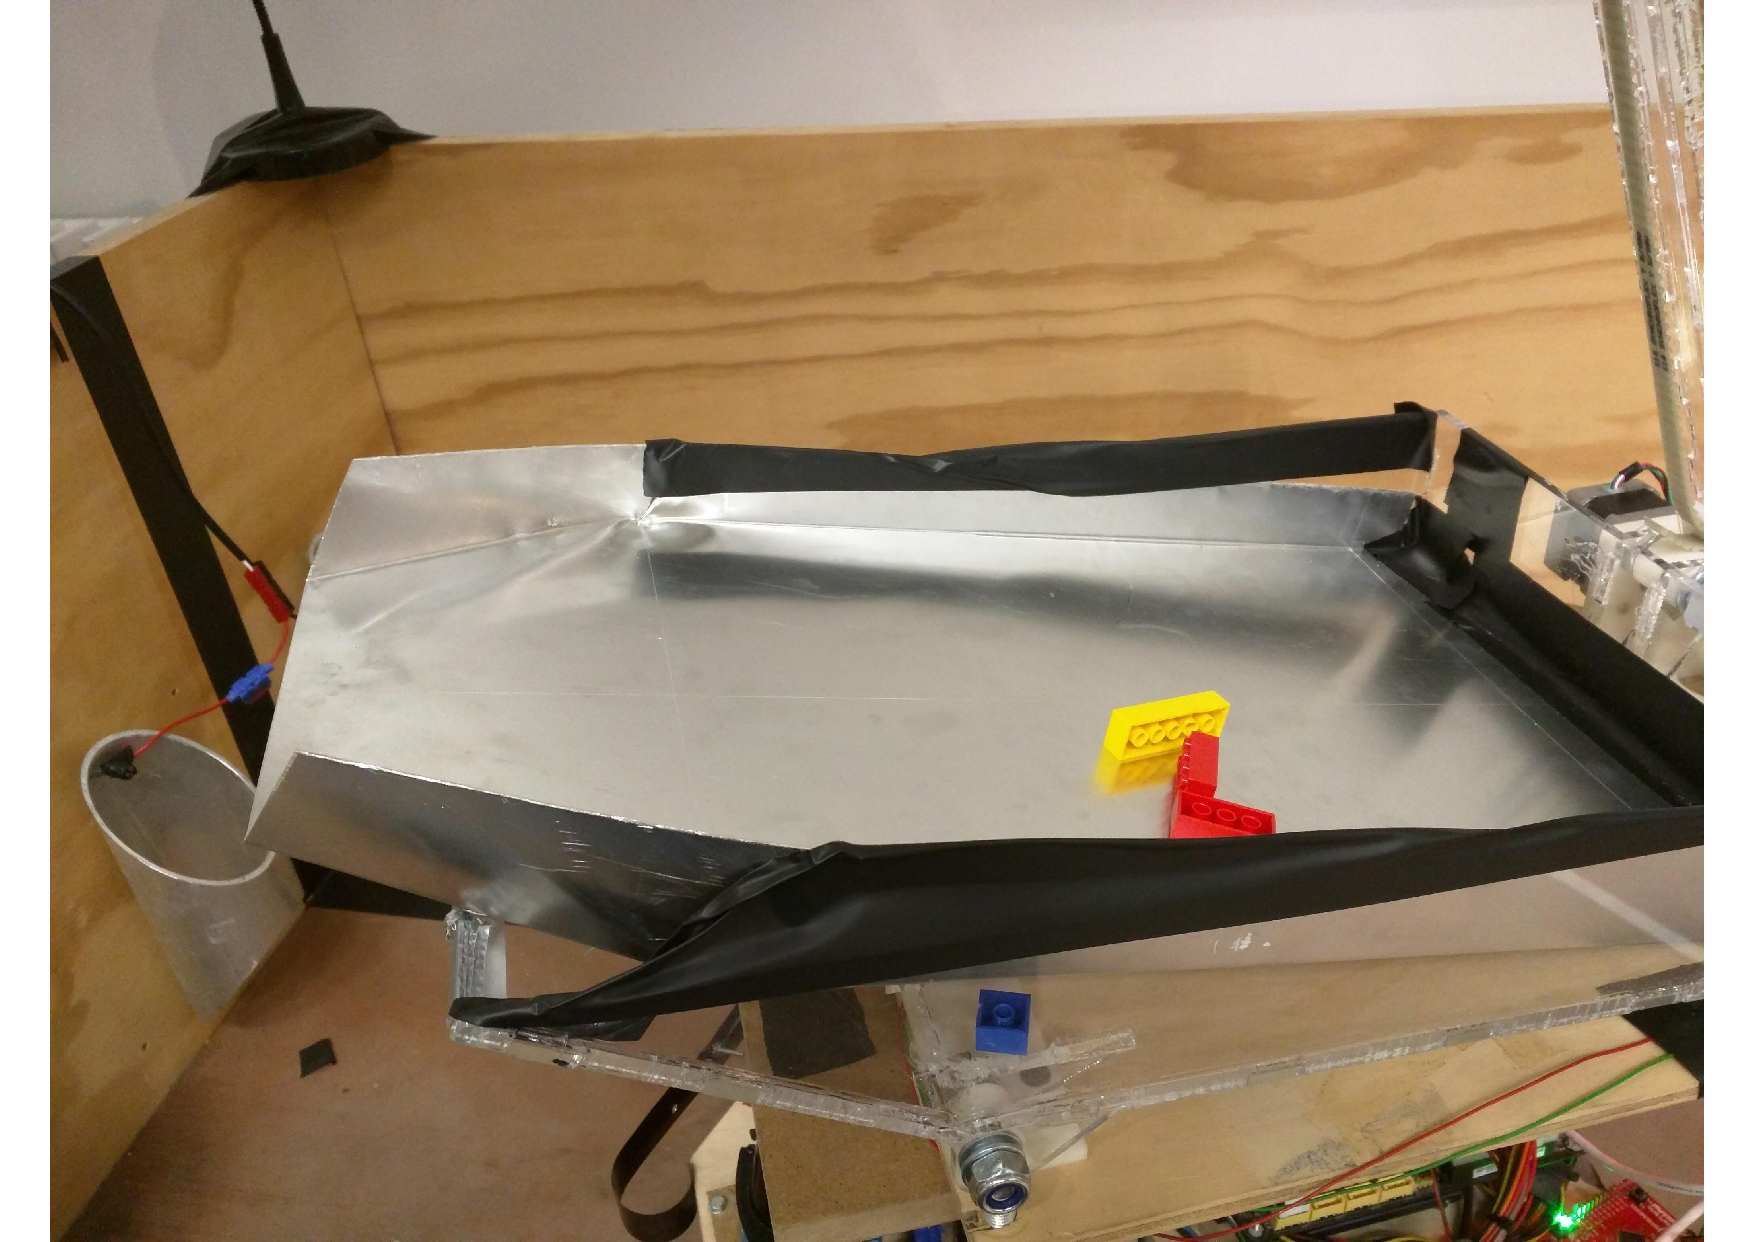
\includegraphics[width=0.7\textwidth]{trayside}
	\caption{Aluminium tray insert on the mobile robot}
	\label{fig:tray}
\end{figure}

% section hardware (end)